% MuniCoins — Technical Whitepaper (Overleaf-compatible)
% Lives at repository root. Upload this file as main.tex or set as root in Overleaf. Compiler: pdfLaTeX or XeLaTeX.
\documentclass[11pt,a4paper]{article}

\usepackage[utf8]{inputenc}
\usepackage[T1]{fontenc}
\usepackage{lmodern}
\usepackage{microtype}
\usepackage[margin=1in]{geometry}
\usepackage{amsmath,amssymb,mathtools}
\usepackage{booktabs}
\usepackage{graphicx}
\usepackage{enumitem}
\usepackage[nameinlink,noabbrev]{cleveref}
\usepackage{hyperref}
\hypersetup{colorlinks=true,linkcolor=blue,urlcolor=blue,citecolor=blue}

\usepackage{tikz}
\usetikzlibrary{arrows.meta,positioning,fit,calc,shapes.multipart}

\usepackage{pgfplots}
\pgfplotsset{compat=1.18}

\title{MuniCoins Technical Whitepaper\\\large Token Valuation Ledger, Intersect Valuation, and Operational Security}
\author{The Mapleseed Incorporated}
\date{\today}

\newcommand{\WAD}{\mathrm{WAD}}
\newcommand{\minor}{\text{minor units}}

\begin{document}
\maketitle

\begin{abstract}
This document supersedes earlier single-track specifications. The platform combines
\textbf{three coupled descriptions}: (I)~the \emph{economic specification} of bifurcated capital and compounding returns;
(II)~the \emph{on-chain ledger encoding} in fixed-point (WAD) form (including a \textbf{global-index reference model});
and (III)~the \emph{Intersect} layer, which combines ledger-derived fair value with NFT-attested and external legs using selectable fusion rules. The \textbf{Introduction} further specifies a \textbf{dual-series system}---\textbf{Series~A} (Accumulation) and \textbf{Series~T} (Treasury)---which may be deployed as \textbf{two separate contracts}, with \textbf{per-token} (NFT-style) state, \textbf{cohort-level} issuance rates for Series~A, and Treasury-bill--style mechanics for Series~T, plus tracking of \textbf{cross-series and FX differentials}. We prove the
specification-to-ledger correspondence under the global-index model, summarize trust boundaries
(issuance authority, Rust EIP-712 sidecar with optional source-network policy, RPC), and reference operational checklists maintained alongside
this repository. \textbf{The core mathematics in Sections~2--4} (economic spec, global-index WAD ledger, Intersect fusion) \textbf{remain the reference encoding for the deployed \texttt{TokenValuationLedger}.} \textbf{Sections~5--7} give the \textbf{fully expanded dual-series formalism}: cohort-indexed Series~A accumulation, Treasury-bill--style Series~T discount and redemption, and cross-series normalization for analytics and Intersect.
\end{abstract}

\tableofcontents
\newpage

%==============================================================================
\section{Introduction}
%==============================================================================

The original algorithmic specification described a single coherent financial model: operational
funds, a frozen premium reserve, per-token activation, compounding fund returns, redemption, and
reissuance. Implementation on Ethereum (\texttt{TokenValuationLedger}) introduces a second,
\emph{machine-oriented} formula system: all monetary amounts live in integer \minor{} of a settlement
asset (e.g.\ USDC), and compounding is tracked via a single global factor in $\WAD=10^{18}$ scale.

Off-chain analytics and pricing APIs may additionally run an \emph{Intersect} engine: two valuations
(a ledger fair value and an NFT-adjusted mirror value) are fused---weighted average, geometric mean,
harmonic mean, or ledger-only---to produce a correlated quote. This yields \textbf{two interacting
formula systems at the product level}: (1)~specification $\leftrightarrow$ chain encoding, and
(2)~ledger leg $\leftrightarrow$ NFT leg within Intersect.

\paragraph{Stability of on-chain economics.}
The \textbf{smart-contract algorithms} (global WAD index, per-slot valuation, policy hooks) and the
\textbf{economic structure} above---bifurcated operational vs.\ premium pools, slot activation, compounding, redemption/reissuance---are \textbf{unchanged} by revisions to off-chain services. Readers sometimes describe the \textbf{paired} ledger leg + mirror leg informally as ``ETF-style'' \emph{coupling}; this document does \emph{not} assert a regulated ETF product. The authoritative relationship remains the mathematics and Solidity interfaces referenced here and in \texttt{contracts/}.

\paragraph{Per-token slots.}
Each position is a distinct integer \textbf{token ID} (a \emph{slot}): transferable, with its own \texttt{active} flag, activation timestamp, and activation-index snapshot; state persists until \textbf{redemption} (payout, slot marked inactive) or until policy-driven \textbf{reissuance} paths apply. Optional \textbf{NFT anchoring} links a slot to an external collection/token id and an \textbf{expected expiry} used to gate some reissue flows---a \emph{claim window}, not (in the reference valuation function) an automatic calendar ``maturity'' that stops accrual by itself. In the \textbf{reference} \texttt{TokenValuationLedger}, \textbf{while active}, every slot reprices against the \textbf{same global compounding index} (period returns posted under governance). \emph{Redeeming} crystallizes value at the then-current index. In a \textbf{multi-cohort Series~A} deployment, repricing uses the cohort index $G^{(c(i))}_t$ in \eqref{eq:series-a-value} instead.

\subsection*{Target system: Series \textbf{A}, Series \textbf{T}, cohorts, and differentials}

The \textbf{intended product architecture} is a \textbf{single integrated system} that may comprise \textbf{two separate on-chain instruments} (two contracts or clearly partitioned deployments), each with \textbf{NFT-style unique token IDs} and full \textbf{per-position} state on the ledger (issue, accrual or discount schedule, redemption, cash-in).

\paragraph{Series \textbf{A} (Accumulation).}
Series~A tokens \textbf{accrue} value while outstanding. A \textbf{batch issuance} (e.g.\ one million tokens) carries parameters fixed at \textbf{that issuance}---notably the \textbf{interest or index rule} for that \textbf{cohort}: all tokens in the batch \textbf{share the same accrual schedule} as one another. A \textbf{later} issuance of another batch (e.g.\ another million) may use a \textbf{different} rate or rule; the system must record \textbf{vintage / cohort} per token ID so redemption and valuation always use the correct schedule. (This goes beyond a single global return curve for all slots unless a deployment explicitly maps cohorts onto one curve.)

\paragraph{Series \textbf{T} (Treasury-style bills).}
Series~T is designed to behave analogously to \textbf{U.S.\ Treasury bills}---short obligations with well-defined \textbf{maturity} and \textbf{cash settlement}---while each position remains a \textbf{distinct NFT-style ID}. \textbf{Cashing in} (redemption at maturity or permitted windows) is supported; the \textbf{ledger records} each settlement. This document does \emph{not} claim U.S.\ government backing or a regulated government security; it describes \textbf{economic analogy} and on-chain mechanics.

\paragraph{Cross-series and external differentials.}
The \textbf{Intersect} layer and system-level analytics are intended to track \textbf{differentials on an individual basis}: between Series~A and Series~T conventions, and relative to \textbf{other system and external references} (e.g.\ settlement in USD vs.\ exposure expressed vs.\ ETH or other legs) where oracles or mirrors are wired. That supports portfolio and risk views across \textbf{instruments and currencies}.

\paragraph{Reference \texttt{TokenValuationLedger} vs.\ this system.}
The repository may include a \textbf{reference} \texttt{TokenValuationLedger} using \textbf{one global compounding index} for all active slots (\cref{sec:wad-ledger}). The \textbf{mathematics} for multi-cohort Series~A and bill-style Series~T is specified in \cref{sec:series-a,sec:series-t,sec:cross-series}. \textbf{On-chain}, full realization of dual-contract Series~A (multi-vintage) and Series~T (bill-style) schedules requires \textbf{additional or successor contracts} and explicit migration; until then, the reference contract serves as a simplified proving ground.

%==============================================================================
\section{System I --- Economic specification}
%==============================================================================

\subsection{Parameters and state}

Let $N$ be total logical token slots, $N_{\mathrm{active}}$ the count of initially active slots,
and inactive slots $N - N_{\mathrm{active}}$ at inception. Prices $P_{\mathrm{initial}}$,
$P_{\mathrm{sale}}$, $P_{\mathrm{core}}$, $P_{\mathrm{premium}}$ satisfy
$P_{\mathrm{sale}} = P_{\mathrm{core}} + P_{\mathrm{premium}}$ and
$P_{\mathrm{initial}} = P_{\mathrm{core}}$ in the reference design.

Operational fund and premium reserve targets follow the bifurcated structure:
\begin{align}
F_{\mathrm{op}} &= P_{\mathrm{core}} \cdot \bigl(N - N_{\mathrm{active}}\bigr), \\
F_{\mathrm{res}} &= P_{\mathrm{premium}} \cdot \bigl(N - N_{\mathrm{active}}\bigr).
\end{align}

For each slot $i$, let $s_i \in \{0,1\}$ indicate inactive/active, $t_i$ activation time, and
$v_i(t)$ economic value at time $t$ for an active token. Fund returns between period boundaries are
encoded by rates $R(t_{k-1},t_k)$. The reference valuation is
\begin{equation}
\label{eq:spec-valuation}
v_i(t) = P_{\mathrm{initial}} \prod_{k\,:\,t_i \le t_k \le t} \bigl(1 + R(t_{k-1},t_k)\bigr),
\end{equation}
for active tokens, with redemption reducing the operational fund by $v_i$ at redemption time and
reissuance resetting the slot to $P_{\mathrm{initial}}$ at a new activation anchor.

\subsection{Earnings}

For an active token over $[t_1,t_2]$,
\begin{equation}
\mathrm{Earnings}_i(t_1,t_2) = v_i(t_1)\, R(t_1,t_2).
\end{equation}

%==============================================================================
\section{System II --- On-chain WAD ledger encoding}
\label{sec:wad-ledger}
%==============================================================================

\subsection{Discrete compounding index}

On-chain arithmetic uses integers. Let $r_t \in \mathbb{Z}$ denote the per-period return encoded in
$\WAD$ such that the multiplicative factor for that period is $(\WAD + r_t)/\WAD$. The global
cumulative factor $G_t$ (contract: \texttt{cumulativeFactorWad}) satisfies $G_0 = \WAD$ and
\begin{equation}
\label{eq:wad-recurrence}
G_{t} = \left\lfloor \frac{G_{t-1} \cdot (\WAD + r_t)}{\WAD} \right\rfloor
\end{equation}
(with Solidity semantics matching the deployed contract). Conceptually, in real numbers,
\begin{equation}
\label{eq:wad-product}
\frac{G_t}{\WAD} = \prod_k \left(1 + \frac{r_k}{\WAD}\right),
\end{equation}
aligning \eqref{eq:wad-product} with \eqref{eq:spec-valuation} when $R_k = r_k/\WAD$.

\subsection{Per-slot activation index}

Each active slot stores an activation index $H_i = G_{t_i}$ (\texttt{indexAtActivationWad}) at
(re)activation time $t_i$. The contract value (in asset minor units, with $P_{\mathrm{initial}}$ in
the same units) is
\begin{equation}
\label{eq:slot-value}
v_i^{\mathrm{chain}} = \left\lfloor \frac{P_{\mathrm{initial}} \cdot G_t}{H_i} \right\rfloor,
\end{equation}
which is the standard global-index trick avoiding per-period iteration at read time.

\subsection{Mapping between System I and System II}

Under a single global return series applied to all active slots, \eqref{eq:spec-valuation} and
\eqref{eq:slot-value} describe the same compounding semantics: \eqref{eq:spec-valuation} is the
continuous product form; \eqref{eq:slot-value} is the ratio form using the same cumulative index.
Rounding and solvency guards (\cref{sec:policies}) introduce bounded implementation differences that
must be monitored by auditors and indexers.

\begin{figure}[htbp]
\centering
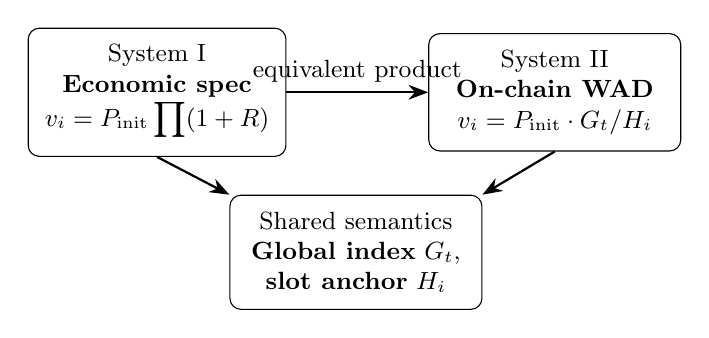
\begin{tikzpicture}[
  font=\small,
  box/.style={draw,rounded corners,align=center,inner sep=6pt,minimum width=3.2cm},
  arr/.style={-{Stealth[length=2.5mm]},thick}
]
\node[box] (spec) {System I\\\textbf{Economic spec}\\$\displaystyle v_i = P_{\mathrm{init}} \prod (1+R)$};
\node[box,right=1.8cm of spec] (wad) {System II\\\textbf{On-chain WAD}\\$\displaystyle v_i = P_{\mathrm{init}} \cdot G_t / H_i$};
\node[box,below=1.3cm of $(spec)!0.5!(wad)$] (idx) {Shared semantics\\\textbf{Global index} $G_t$,\\\textbf{slot anchor} $H_i$};
\draw[arr] (spec) -- node[above]{equivalent product} (wad);
\draw[arr] (spec.south) -- (idx.north west);
\draw[arr] (wad.south) -- (idx.north east);
\end{tikzpicture}
\caption{Specification valuation (product of returns) and on-chain valuation (ratio of cumulative
factors) share one global compounding process.}
\label{fig:spec-chain}
\end{figure}

%==============================================================================
\section{System III --- Intersect dual-leg valuation}
\label{sec:intersect}
%==============================================================================

The Intersect module (\texttt{src/intersect/}) fuses two \emph{sources} of value:

\begin{itemize}[leftmargin=*]
  \item \textbf{Ledger leg} $L$: fair value from the on-chain ledger model, expressed in a \textbf{common numeraire} (e.g.\ USD \minor). Instantiations include the reference global-index slot value \eqref{eq:slot-value}, the Series~A cohort value \eqref{eq:series-a-value}, or Series~T economic value before maturity \eqref{eq:series-t-linear}--\eqref{eq:series-t-pv} or face at maturity \eqref{eq:series-t-maturity}.
  \item \textbf{NFT leg} $N$: an NFT-attested mirror value, adjusted by a leg multiplier in $\WAD$.
\end{itemize}

Let $N' = (N_{\mathrm{raw}} \cdot m)/\WAD$ with multiplier $m$ (\texttt{legMultiplierWad}). Modes:

\paragraph{Ledger-primary.}
$\mathrm{combined} = L$.

\paragraph{Weighted.}
With weights $w_L, w_N$ in basis points summing to $10{,}000$,
\begin{equation}
\mathrm{combined} = \frac{w_L\, L + w_N\, N'}{10{,}000}.
\end{equation}

\paragraph{Geometric.}
\begin{equation}
\mathrm{combined} = \left\lfloor \sqrt{L \cdot N'} \right\rfloor \quad \text{(integer square root as implemented).}
\end{equation}

\paragraph{Cross-coupled (harmonic).}
For $L, N' > 0$,
\begin{equation}
\mathrm{combined} = \left\lfloor \frac{2\, L\, N'}{L + N'} \right\rfloor .
\end{equation}

Optional \emph{relaxation} iterates a midpoint map until convergence:
$(a,b) \mapsto \bigl\lfloor (a+b)/2 \bigr\rfloor$ with stopping on $\epsilon$.

\begin{figure}[htbp]
\centering
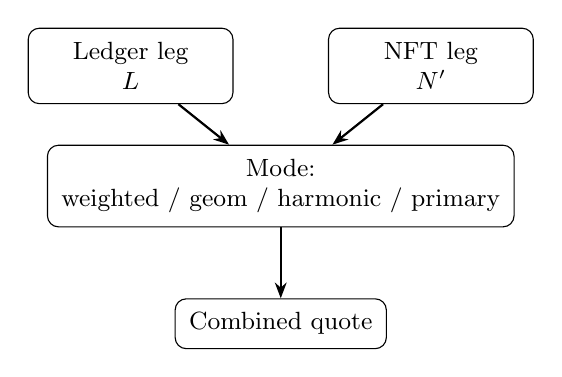
\begin{tikzpicture}[
  font=\small,
  box/.style={draw,rounded corners,inner sep=5pt,minimum width=2.6cm,align=center},
  arr/.style={-{Stealth[length=2mm]},thick}
]
\node[box] (L) {Ledger leg\\$L$};
\node[box,right=1.2cm of L] (N) {NFT leg\\$N'$};
\node[box,below=1.0cm of $(L)!0.5!(N)$] (M) {Mode:\\weighted / geom / harmonic / primary};
\node[box,below=0.9cm of M] (Q) {Combined quote};
\draw[arr] (L) -- (M);
\draw[arr] (N) -- (M);
\draw[arr] (M) -- (Q);
\end{tikzpicture}
\caption{Intersect combines two valuation systems (ledger vs NFT-attested mirror) into one quoted amount.}
\label{fig:intersect}
\end{figure}

%==============================================================================
\section{System IV --- Series A: cohort-indexed accumulation}
\label{sec:series-a}
%==============================================================================

Series~A positions \textbf{accrue} while outstanding. Unlike the reference single-index model (\cref{sec:wad-ledger}), each \textbf{issuance batch} (cohort) may carry its own compounding rule. All tokens minted in the same batch share one \textbf{cohort id} $c \in \{1,\ldots,C\}$; tokens carry an immutable assignment $c(i)$ at mint.

\subsection{Cohort compounding indices (economic form)}

Fix a cohort $c$. Let $\tau_c$ be the cohort inception time (first period when that cohort's index is defined). Between governance period boundaries $t_{k-1}, t_k$ with $\tau_c \le t_{k-1}$, let $R^{(c)}(t_{k-1},t_k)$ denote the \textbf{cohort-specific} period return for cohort $c$. For an active token $i$ with $c(i)=c$, activation time $t_i \ge \tau_c$, and $t \ge t_i$,
\begin{equation}
\label{eq:series-a-spec}
v_i(t) = P^{(c)}_{\mathrm{initial}}
\prod_{k\,:\,t_i \le t_k \le t}
\bigl(1 + R^{(c)}(t_{k-1},t_k)\bigr),
\end{equation}
where $P^{(c)}_{\mathrm{initial}}$ is the cohort's principal anchor (economic parameter). Different cohorts $c \neq c'$ may use different sequences $R^{(c)}$ and $R^{(c')}$. If all slots share one cohort and one global return series, \eqref{eq:series-a-spec} collapses to \eqref{eq:spec-valuation}.

\subsection{On-chain WAD encoding per cohort}

For each cohort $c$, maintain a \textbf{cumulative WAD factor} $G^{(c)}_t$ with $G^{(c)}_{\tau_c} = \WAD$ (or an equivalent fixed anchor chosen at deployment). Let $r^{(c)}_t \in \mathbb{Z}$ encode the posted period return for cohort $c$ in period $t$ in the same $\WAD$ convention as \eqref{eq:wad-recurrence}. Then
\begin{equation}
\label{eq:series-a-wad-recurrence}
G^{(c)}_{t} = \left\lfloor \frac{G^{(c)}_{t-1} \cdot (\WAD + r^{(c)}_t)}{\WAD} \right\rfloor,
\qquad t > \tau_c .
\end{equation}
Token $i$ with cohort $c(i)$ stores an activation snapshot $H_i = G^{(c(i))}_{t_i}$. The on-chain Series~A value is
\begin{equation}
\label{eq:series-a-value}
v_i^{\mathrm{chain},A} = \left\lfloor \frac{P^{(c(i))}_{\mathrm{initial}} \cdot G^{(c(i))}_t}{H_i} \right\rfloor,
\end{equation}
in settlement \minor, matching the same ratio trick as \eqref{eq:slot-value} but with a \textbf{cohort-indexed} factor. Redemption crystallizes $v_i^{\mathrm{chain},A}$ at the then-current $G^{(c(i))}_t$ and $t$.

\subsection{Earnings and mapping}

Cohort earnings over $[t_1,t_2]$ follow the same structural identity as System~I with cohort-subscripted rates:
\begin{equation}
\mathrm{Earnings}^{(c)}_i(t_1,t_2) = v_i(t_1)\, R^{(c)}(t_1,t_2).
\end{equation}
Under one cohort and identical posting of $r_t = r^{(c)}_t$, \eqref{eq:series-a-value} and \eqref{eq:slot-value} coincide up to notation.

%==============================================================================
\section{System V --- Series T: Treasury-bill-style discount instruments}
\label{sec:series-t}
%==============================================================================

Series~T positions are \textbf{short obligations} with \textbf{face value}, \textbf{issue price}, and \textbf{maturity}. Each token id $i$ carries: face $F_i > 0$ and issue price $P^{\mathrm{issue}}_i$ (both in settlement \minor), issue time $t^{\mathrm{issue}}_i$, and maturity $T_i > t^{\mathrm{issue}}_i$. Typically $P^{\mathrm{issue}}_i \le F_i$ (discount issuance). This document states \textbf{economic analogy} to U.S.\ T-bills; it does not assert sovereign or regulated-product status.

\subsection{Linear accretion (primary reference schedule)}

Between issue and maturity, define the \textbf{accreted economic value} by linear interpolation from issue price to face:
\begin{equation}
\label{eq:series-t-linear}
v_i^{\mathrm{econ},T}(t) =
\begin{cases}
P^{\mathrm{issue}}_i
+ (F_i - P^{\mathrm{issue}}_i)\,
\dfrac{t - t^{\mathrm{issue}}_i}{T_i - t^{\mathrm{issue}}_i},
& t^{\mathrm{issue}}_i \le t < T_i, \\[0.8em]
F_i, & t \ge T_i \quad \text{and not yet redeemed,}
\end{cases}
\end{equation}
with redemption recording a payout of $F_i$ (or policy-permitted variant) and marking the position settled. Implementations may replace linear accretion with a \textbf{step schedule} tied to posted period boundaries; the \textbf{ledger invariant} is that at $T_i$ the outstanding claim equals $F_i$ before cash-in.

\subsection{Discount yields (quoting conventions)}

For discount instruments it is common to quote a \textbf{bank discount yield} on a $F$-par, $P$-price, $n$-day instrument (symbolic; day-count conventions vary):
\begin{equation}
\label{eq:bank-discount}
Y_d = \frac{F_i - P^{\mathrm{issue}}_i}{F_i} \cdot \frac{360}{n},
\end{equation}
and a \textbf{bond-equivalent} or \textbf{money-market} yield for comparison across products. These are \textbf{reporting} identities; on-chain settlement uses integer \minor{} and the schedule in \eqref{eq:series-t-linear} or the contract's posted discrete accretion table.

\subsection{Secondary-style mark (optional, pre-maturity)}

For analytics or Intersect, a \textbf{mark-to-market} before $T_i$ may discount the face at a short rate. Let $y$ denote an annualized simple or continuously compounded short yield appropriate to the horizon $(T_i - t)$ in calendar or ACT/360 form. A continuous-style present value (illustrative) is
\begin{equation}
\label{eq:series-t-pv}
\tilde{v}_i^{T}(t) = F_i\, e^{-y\,(T_i - t)},
\qquad t < T_i,
\end{equation}
with $y$ sourced from an oracle or curve. \eqref{eq:series-t-pv} is \textbf{not} required to match \eqref{eq:series-t-linear}; reconciling \emph{book} (accretion) vs \emph{market} (discount) legs is an Intersect or risk-system concern.

\subsection{Maturity and ledger cash-in}

At or after $T_i$, the holder may \textbf{cash in} for
\begin{equation}
\label{eq:series-t-maturity}
\mathrm{payout}_i = F_i \quad \text{(minus fees if policy applies).}
\end{equation}
The ledger emits settlement events so indexers record \textbf{which} token ids redeemed, preserving a complete history of Series~T cash flows.

%==============================================================================
\section{System VI --- Cross-series normalization and differentials}
\label{sec:cross-series}
%==============================================================================

Portfolio views and Intersect often require \textbf{comparable scalars} across Series~A, Series~T, and external references (e.g.\ ETH notional).

\subsection{Common numeraire}

Let $\mathcal{N}$ denote a chosen settlement asset (e.g.\ USD stablecoin \minor). Values $v_i^{A}$ from \eqref{eq:series-a-value} are already in $\mathcal{N}$ if $P^{(c)}_{\mathrm{initial}}$ and factors are posted in $\mathcal{N}$. Series~T values use $v_i^{\mathrm{econ},T}(t)$ from \eqref{eq:series-t-linear} or marks $\tilde{v}_i^{T}(t)$ from \eqref{eq:series-t-pv} in the same $\mathcal{N}$ when face and issue prices are in $\mathcal{N}$.

\subsection{FX or secondary legs}

Let $X$ denote an amount in another asset (e.g.\ ETH in wei). Given an oracle price $\Pi_{\mathcal{N}/X}$ (units of $\mathcal{N}$ per one unit of $X$), define the \textbf{converted} value $\mathrm{conv}(X) = X \cdot \Pi_{\mathcal{N}/X}$ in \minor{} after fixed-point scaling consistent with the oracle feed.

\subsection{Pairwise differentials}

For two positions $i,j$ (same or different series) with comparable values $\hat{v}_i,\hat{v}_j$ in $\mathcal{N}$,
\begin{equation}
\label{eq:differential}
\Delta_{i,j} = \hat{v}_i - \hat{v}_j .
\end{equation}
Series tags and cohort ids are carried in metadata so analytics can aggregate $\Delta$ across baskets (e.g.\ cohort $c$ vs cohort $c'$) or Series~A vs Series~T sleeves.

\subsection{Intersect with heterogeneous ledger legs}

Intersect (\cref{sec:intersect}) consumes a single ledger leg $L$. In multi-series deployments, \textbf{choose} $L$ from the appropriate formula: \eqref{eq:series-a-value} for Series~A token $i$, or \eqref{eq:series-t-linear} / \eqref{eq:series-t-pv} / \eqref{eq:series-t-maturity} for Series~T depending on product mode (accrual book vs mark). The fusion rules in Section~4 then combine that $L$ with the NFT leg $N'$ unchanged.

%==============================================================================
\section{Architecture and trust boundaries (summary)}
%==============================================================================

\begin{figure}[htbp]
\centering
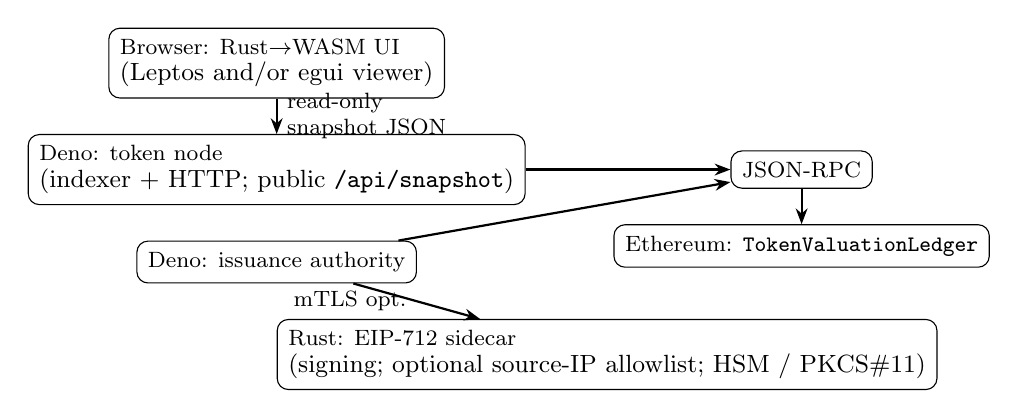
\begin{tikzpicture}[
  font=\footnotesize,
  box/.style={draw,rounded corners,inner sep=4pt,align=left},
  arr/.style={-{Stealth[length=2mm]},thick}
]
\node[box] (browser) {Browser: Rust$\to$WASM UI\\\small (Leptos and/or egui viewer)};
\node[box,below=0.45cm of browser] (toknode) {Deno: token node\\\small (indexer + HTTP; public \texttt{/api/snapshot})};
\node[box,below=0.45cm of toknode] (auth) {Deno: issuance authority};
\node[box,below=0.45cm of auth,anchor=north west] (sidecar) {Rust: EIP-712 sidecar\\\small (signing; optional source-IP allowlist; HSM / PKCS\#11)};
\node[box,right=2.6cm of toknode] (rpc) {JSON-RPC};
\node[box,below=0.45cm of rpc] (chain) {Ethereum: \texttt{TokenValuationLedger}};
\draw[arr] (browser) -- node[right,align=left]{\footnotesize read-only\\\footnotesize snapshot JSON} (toknode);
\draw[arr] (auth) -- node[left]{mTLS opt.} (sidecar);
\draw[arr] (auth) -- (rpc);
\draw[arr] (toknode) -- (rpc);
\draw[arr] (rpc) -- (chain);
\end{tikzpicture}
\caption{Simplified trust boundaries: WASM UIs consume public chain mirrors from the token node; issuance may call the Rust sidecar for signing; all rely on RPC for chain state (see \texttt{docs/security/threat-model.md}).}
\label{fig:arch}
\end{figure}

\noindent
Full operational procedures (rotation, ceremonies, logging, runbooks, backups) are in
\texttt{docs/security/operational-controls.md}. Threat modeling and RPC/sidecar compromise scenarios:
\texttt{docs/security/threat-model.md}. mTLS between issuance authority and sidecar:
\texttt{docs/security/mtls-authority-sidecar.md}. Deployment parameter checklist:
\texttt{docs/deployment/environment-checklist.md}.

%==============================================================================
\section{On-chain policy hooks (reference)}
\label{sec:policies}

The ledger exposes policy setters (role-gated): issuance certification (\texttt{setIssuanceCertificationPolicy}),
solvency (\texttt{setSolvencyPolicy}), expiry proofs, compliance mode, pausing, return-period replay
protection, and others. Exact selectors and events appear in \texttt{contracts/TokenValuationLedger.sol}.

%==============================================================================
\appendix

\section{Numeric illustration (Intersect)}

Let $L=100$, $N'=64$. Weighted $70/30$ gives $0.7\cdot 100 + 0.3\cdot 64 = 89.2$.
Geometric mean $\sqrt{100\cdot 64}=80$. Harmonic $2\cdot100\cdot64/(100+64)\approx 78.05$.

\begin{center}
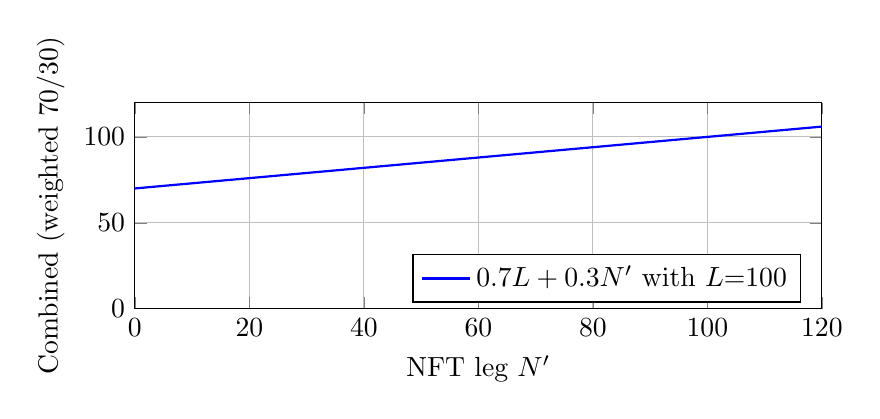
\begin{tikzpicture}
\begin{axis}[
  width=0.85\linewidth,
  height=4.2cm,
  xlabel={NFT leg $N'$},
  ylabel={Combined (weighted 70/30)},
  xmin=0, xmax=120,
  ymin=0, ymax=120,
  grid=both,
  legend pos=south east
]
\addplot[thick,blue,domain=0:120] {0.7*100 + 0.3*x};
\addlegendentry{$0.7 L + 0.3 N'$ with $L{=}100$}
\end{axis}
\end{tikzpicture}
\end{center}

\section{Numeric illustration (Series A and Series T)}

\paragraph{Series A (two cohorts, ratio read).}
Suppose cohort $c=1$ has $P^{(1)}_{\mathrm{initial}}=100$ and at read time $G^{(1)}_t / \WAD = 1.05$, with activation snapshot $H_i/\WAD = 1.00$. Then $v_i^{\mathrm{chain},A} \approx \lfloor 100 \cdot 1.05 / 1.00\rfloor = 105$ in \minor{} (ignoring flooring detail). A \textbf{later} cohort $c=2$ may post a different factor $G^{(2)}_t$; tokens with $c(i)=2$ use \eqref{eq:series-a-value} with $G^{(c(2))}$ only.

\paragraph{Series T (linear accretion).}
Let $F_i=1000$, $P^{\mathrm{issue}}_i=980$, $t^{\mathrm{issue}}_i=0$, $T_i=1$ in arbitrary time units. At $t=0.5$, \eqref{eq:series-t-linear} gives $v_i^{\mathrm{econ},T}(0.5) = 980 + 20 \cdot 0.5 = 990$. At $t \ge 1$ before redemption, economic value is $1000$; cash-in pays \eqref{eq:series-t-maturity} with payout $1000$.

\section{Frontend and build tooling (non-normative)}

The repository ships \textbf{Rust$\to$WASM} read-only dashboards: a \textbf{Leptos} CSR app in \texttt{ui/} (built with Trunk; static files may be served by Deno or any static host) and a legacy \textbf{egui} viewer in \texttt{viewer-egui/}. Neither changes on-chain rules; security depends on avoiding embedded secrets, validating API inputs, HTTPS, and CORS policy. Unified build entrypoints: \texttt{BUILD.md}, \texttt{justfile}, and \texttt{scripts/build.sh}. See \texttt{docs/frontend-architecture.md} and \texttt{docs/security/hardened-viewer.md} for UI hardening options and limits.

\end{document}
